
Essentially this examines the Pearson correlation between 
shifted version of the indicator and the case rate. So if $X_{\ell,t}$ is
shifted forward by 7 days, and the magnitude of the correlation of that shifted series with
$Y_{\ell,t}$ (unshifted) is high, we would say that $X_{\ell}$ leads $Y_{\ell}$
by 7 days. This process is repeated for a range of shifts, forward and backward,
resulting in leadingness and laggingness scores. Further details are given in
the supplement.

%%%%%

Because a time series can, to a degree, both simultaneously leading and lagging,
we also examine the correlation between performance and the difference between
leadingness and laggingness. Figure \ref{fig:diff-btw-leading-lagging} shows
this behavior. Again, indicators that are more leading then lagging tend to
are positively correlated with improved relative performance. This relationship
is most pronounced during periods of decreasing case rates and attenuates in
other scenarios.


\begin{figure}[t]
  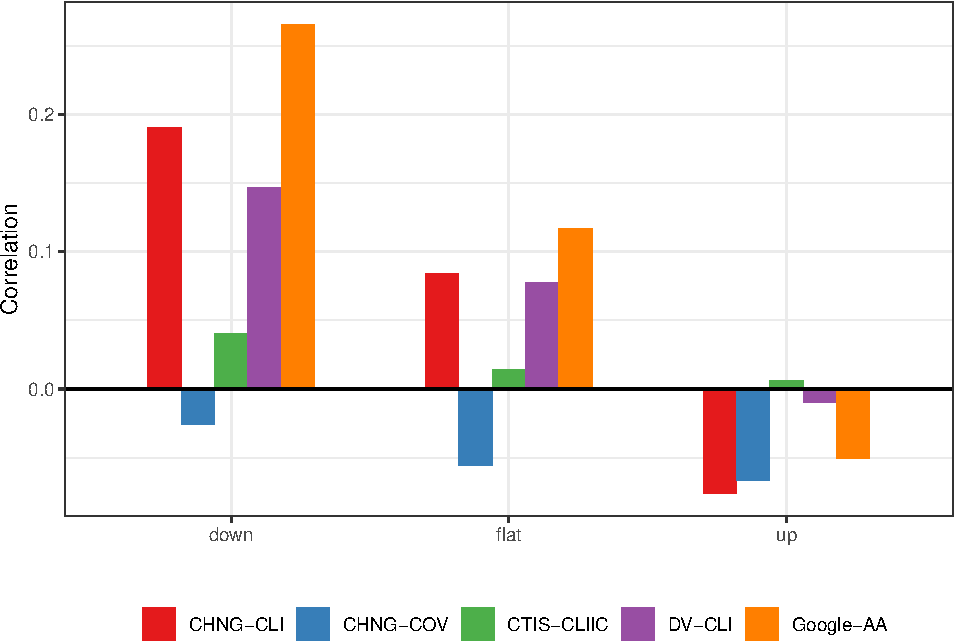
\includegraphics[width=\columnwidth]{fig/diff-in-lead-lag-1.pdf}
  \caption{Correlation of the difference in WIS with difference between the
    ``leadingness'' and ``laggingness'' of the indicator at the target date.}
  \label{fig:diff-btw-leading-lagging}
\end{figure}


%%%%%


We also investigate the effect of lengthening the time window to include 2021. 
\begin{itemize}
\item For forecasting: results get better, whether we look at
  non-adjusted (first plot) or adjusted scores (second plot).  Other
  than that, interpretation is qualitatively similar, except fb now
  seems to be worse than gs.  And \chngcli~is strong, even in the
  non-adjusted view.
  \item For hotspots: Alden will write something explaining why we
    don't do hotspot detection in 2021.
\end{itemize}

%%%%% 

We look at various approaches to
accounting for the fact that the \gs~indicator is only available
for XX HRRs.

\begin{itemize}
  \item For forecasting task: clearly gs is not missing at random, and when it's present, it tends to be predictive.  Hence high values have a low false positivity rate.  Most visible in the adjusted view below, where gs triumphs.  Also \chngcli~gets a lot worse.

\item For hotspots: All methods look better, suggesting that the “GS locations” are easier for hotspot prediction. E.g. at 7-days ahead, the AUCs computed based on all locations range from 0.61-0.66; restricted to GS locations, the AUCs range from about 0.65-0.69. (These are all eyeballed, should get actual numbers if we want to say something like this in paper.)
\item gs\_subset appears to be particularly helped by this subsetting
  (which makes sense since on those other locations it was 0-imputed)
  \item Daniel will also try gs\_impute as in forecasting
\end{itemize}

%%%%%


